\documentclass[conference]{IEEEtran}
\IEEEoverridecommandlockouts
\usepackage{cite}
\usepackage{amsmath,amssymb}
\usepackage{graphicx}
\usepackage{booktabs}
\usepackage{multirow}
\usepackage{xcolor}
\usepackage[hidelinks]{hyperref}

% Every number in the prose comes from tables/numbers.tex, generated by make_tables.py.
% Generated by make_tables.py. Do not edit.
\newcommand{\cpuCount}{8}
\newcommand{\cupKnnAccuracy}{99.88}
\newcommand{\cupKnnPrecision}{99.93}
\newcommand{\cupKnnRecall}{99.92}
\newcommand{\cupNbAccuracy}{98.72}
\newcommand{\cupNbPrecision}{99.43}
\newcommand{\cupNbRecall}{98.96}
\newcommand{\diffKnnAccuracy}{5.24}
\newcommand{\diffKnnPrecision}{2.39}
\newcommand{\diffKnnRecall}{10.42}
\newcommand{\diffNbAccuracy}{1.03}
\newcommand{\diffNbPrecision}{1.56}
\newcommand{\diffNbRecall}{7.98}
\newcommand{\dtPredMax}{1.32}
\newcommand{\dtPredMin}{0.39}
\newcommand{\forestAboveSvmN}{2}
\newcommand{\knnLoaoMax}{1.79}
\newcommand{\knnPredCupAll}{21.87}
\newcommand{\knnPredMax}{4627.1}
\newcommand{\knnPredMin}{498.9}
\newcommand{\knnPredTopN}{4}
\newcommand{\loaoCupAllRf}{0.97}
\newcommand{\loaoCupAllRft}{28.84}
\newcommand{\loaoCupAllSvm}{0.00}
\newcommand{\loaoCupEightRf}{23.78}
\newcommand{\loaoCupEightRft}{17.69}
\newcommand{\loaoCupEightSvm}{19.35}
\newcommand{\loaoFaMax}{0.64}
\newcommand{\loaoN}{80}
\newcommand{\loaoNslAllRf}{2.18}
\newcommand{\loaoNslAllRft}{0.93}
\newcommand{\loaoNslAllSvm}{0.76}
\newcommand{\loaoNslEightRf}{2.42}
\newcommand{\loaoNslEightRft}{0.47}
\newcommand{\loaoNslEightSvm}{0.41}
\newcommand{\loaoSeenMin}{95.86}
\newcommand{\loaoUnderHalf}{75}
\newcommand{\meanKnnAccuracy}{93.27}
\newcommand{\meanKnnPrecision}{96.51}
\newcommand{\meanKnnRecall}{87.38}
\newcommand{\meanNbAccuracy}{92.92}
\newcommand{\meanNbPrecision}{96.18}
\newcommand{\meanNbRecall}{87.56}
\newcommand{\minAccAllCup}{99.95}
\newcommand{\minAccAllHold}{99.69}
\newcommand{\nCategorical}{3}
\newcommand{\nDosTypes}{10}
\newcommand{\nSetups}{6}
\newcommand{\nbAccAllCup}{93.31}
\newcommand{\nbAccAllHold}{65.78}
\newcommand{\nbAccAllOff}{61.78}
\newcommand{\nbAccEightCup}{98.72}
\newcommand{\nbAccEightHold}{95.52}
\newcommand{\nbAccEightOff}{87.12}
\newcommand{\nbFaMax}{98.92}
\newcommand{\nbLoaoNslAllFa}{45.61}
\newcommand{\nbLoaoNslAllRec}{48.67}
\newcommand{\nbLoaoNslEightFa}{30.87}
\newcommand{\nbLoaoNslEightRec}{36.46}
\newcommand{\nbSmurfCupFa}{6.98}
\newcommand{\nbSmurfCupRec}{99.99}
\newcommand{\nbSmurfNslFa}{98.92}
\newcommand{\nbSmurfNslRec}{100.00}
\newcommand{\nslKnnAccuracy}{86.66}
\newcommand{\nslKnnPrecision}{93.09}
\newcommand{\nslKnnRecall}{74.83}
\newcommand{\nslNbAccuracy}{87.12}
\newcommand{\nslNbPrecision}{92.93}
\newcommand{\nslNbRecall}{76.15}
\newcommand{\offAccAllDt}{91.33}
\newcommand{\offAccAllRf}{90.12}
\newcommand{\offAccAllRft}{90.59}
\newcommand{\offAccAllSvm}{93.03}
\newcommand{\offAccDtAll}{91.33}
\newcommand{\offAccDtEight}{84.97}
\newcommand{\offAccKnnAll}{89.53}
\newcommand{\offAccKnnEight}{86.66}
\newcommand{\offAccNbAll}{61.78}
\newcommand{\offAccNbEight}{87.12}
\newcommand{\offAccSvmAll}{93.03}
\newcommand{\offAccSvmEight}{86.76}
\newcommand{\offFoneDtAll}{89.28}
\newcommand{\offFoneDtEight}{80.39}
\newcommand{\offFoneKnnAll}{86.41}
\newcommand{\offFoneKnnEight}{82.97}
\newcommand{\offFoneNbAll}{65.10}
\newcommand{\offFoneNbEight}{83.71}
\newcommand{\offFoneSvmAll}{91.34}
\newcommand{\offFoneSvmEight}{83.14}
\newcommand{\paperKnnAcc}{98.51}
\newcommand{\paperKnnAccuracy}{98.51}
\newcommand{\paperKnnPrecision}{98.90}
\newcommand{\paperKnnRecall}{97.80}
\newcommand{\paperNbAccuracy}{93.95}
\newcommand{\paperNbPrecision}{97.74}
\newcommand{\paperNbRecall}{95.54}
\newcommand{\pyVersion}{3.12.3}
\newcommand{\rankCupCount}{3}
\newcommand{\rankCupDstBytes}{1}
\newcommand{\rankCupDstHostCount}{4}
\newcommand{\rankCupProtocol}{6}
\newcommand{\rankNslCount}{8}
\newcommand{\rankNslDstBytes}{9}
\newcommand{\rankNslDstHostCount}{15}
\newcommand{\rankNslProtocol}{19}
\newcommand{\repeats}{5}
\newcommand{\rfDefAllCv}{}
\newcommand{\rfDefAllF}{0.8720}
\newcommand{\rfDefAllU}{0.0684}
\newcommand{\rfDefEightCv}{}
\newcommand{\rfDefEightF}{0.8111}
\newcommand{\rfDefEightU}{0.2048}
\newcommand{\rfTrainCupAll}{10.32}
\newcommand{\rfTunAoCv}{0.0797}
\newcommand{\rfTunAoF}{0.8833}
\newcommand{\rfTunAoU}{0.1406}
\newcommand{\rfTunStdCv}{0.9998}
\newcommand{\rfTunStdF}{0.8773}
\newcommand{\rfTunStdU}{0.0978}
\newcommand{\seenDtAll}{98.68}
\newcommand{\seenDtEight}{86.52}
\newcommand{\seenKnnAll}{97.53}
\newcommand{\seenKnnEight}{87.67}
\newcommand{\seenNbAll}{93.36}
\newcommand{\seenNbEight}{85.16}
\newcommand{\seenSvmAll}{98.95}
\newcommand{\seenSvmEight}{86.87}
\newcommand{\skVersion}{1.9.1}
\newcommand{\svmAccEightHold}{97.19}
\newcommand{\svmLoaoFaMax}{0.53}
\newcommand{\svmLoaoMeanMax}{19.35}
\newcommand{\svmLoaoN}{16}
\newcommand{\svmLoaoOverGroup}{\texttt{neptune}}
\newcommand{\svmLoaoOverN}{1}
\newcommand{\svmLoaoOverRec}{69.35}
\newcommand{\svmLoaoOverSetup}{KDDCup with 8 features}
\newcommand{\svmLoaoSeenMin}{95.94}
\newcommand{\svmLoaoUnderHalf}{15}
\newcommand{\svmPredMax}{2731}
\newcommand{\svmPredMin}{98.3}
\newcommand{\svmPredSecMax}{7.5}
\newcommand{\svmPredTopN}{2}
\newcommand{\svmTrainAllMax}{22.4}
\newcommand{\svmTrainAllMin}{1.2}
\newcommand{\svmTrainEightMax}{137.3}
\newcommand{\svmTrainEightMin}{37.1}
\newcommand{\svmTrainRatioMax}{2958}
\newcommand{\svmTrainRatioMin}{4.0}
\newcommand{\svmTrainSecMax}{137.3}
\newcommand{\svmTrainTopN}{4}
\newcommand{\testDosCount}{7{,}458}
\newcommand{\topCup}{\texttt{dst\_\allowbreak bytes}, \texttt{logged\_\allowbreak in}, \texttt{count}, \texttt{dst\_\allowbreak host\_\allowbreak count}, \texttt{dst\_\allowbreak host\_\allowbreak srv\_\allowbreak diff\_\allowbreak host\_\allowbreak rate}, \texttt{protocol\_\allowbreak type}, \texttt{srv\_\allowbreak count}, \texttt{srv\_\allowbreak diff\_\allowbreak host\_\allowbreak rate}}
\newcommand{\topNsl}{\texttt{same\_\allowbreak srv\_\allowbreak rate}, \texttt{flag}, \texttt{diff\_\allowbreak srv\_\allowbreak rate}, \texttt{serror\_\allowbreak rate}, \texttt{srv\_\allowbreak serror\_\allowbreak rate}, \texttt{dst\_\allowbreak host\_\allowbreak serror\_\allowbreak rate}, \texttt{dst\_\allowbreak host\_\allowbreak srv\_\allowbreak serror\_\allowbreak rate}, \texttt{count}}
\newcommand{\trainRfMax}{49.3}
\newcommand{\trainRfMin}{8.8}
\newcommand{\trainRftMax}{60.2}
\newcommand{\trainRftMin}{9.5}
\newcommand{\unseenCount}{1{,}717}
\newcommand{\unseenDtAll}{30.81}
\newcommand{\unseenDtEight}{18.75}
\newcommand{\unseenKnnAll}{6.93}
\newcommand{\unseenKnnEight}{31.92}
\newcommand{\unseenMaxAll}{44.26}
\newcommand{\unseenMaxEight}{46.01}
\newcommand{\unseenMinAll}{6.93}
\newcommand{\unseenMinEight}{18.75}
\newcommand{\unseenNbAll}{44.26}
\newcommand{\unseenNbEight}{46.01}
\newcommand{\unseenRfAll}{8.21}
\newcommand{\unseenRfEight}{19.86}
\newcommand{\unseenRftAll}{26.97}
\newcommand{\unseenRftEight}{29.94}
\newcommand{\unseenShare}{23.02}
\newcommand{\unseenShareOne}{23.0}
\newcommand{\unseenSvmAll}{36.69}
\newcommand{\unseenSvmEight}{36.05}
\newcommand{\unseenSvmRankAll}{2}
\newcommand{\unseenSvmRankEight}{2}
\newcommand{\unseenTopIsNbAll}{yes}
\newcommand{\unseenTopIsNbEight}{yes}

\newcommand{\nm}[1]{\csname #1\endcsname}
\newcommand{\pc}[1]{\csname #1\endcsname\%}

\begin{document}

\title{Reproducing and Extending a KNN and Naive Bayes DoS Detector for Network Forensics: Generalization to Unseen Attack Types}

\author{\IEEEauthorblockN{1\textsuperscript{st} Joshua Gottus}
  \IEEEauthorblockA{\textit{Department of Computer Science} \\
    \textit{Florida Polytechnic University}\\
    Lakeland, USA \\
  jgottus9500@floridapoly.edu}
  \and
  \IEEEauthorblockN{2\textsuperscript{nd} Ethan Barron}
  \IEEEauthorblockA{\textit{Department of Computer Science} \\
    \textit{Florida Polytechnic University}\\
    Lakeland, USA \\
  ebarron5743@floridapoly.edu}
}

\maketitle

\begin{abstract}
Machine learning classifiers are widely proposed for detecting denial-of-service (DoS) attacks in network traffic during forensic investigations, yet reported results are often difficult to verify and rarely examine attacks absent from the training data. We attempt to reproduce a published comparison of K-nearest neighbors and Naive Bayes on the KDDCup'99 and NSL-KDD datasets from its secondary description, and we extend the comparison with a decision tree, a random forest and a tuned random forest. Models were evaluated on three splits, with 8 or 41 features, and under a leave-one-attack-out protocol in which each DoS type is withheld in turn. Our two-dataset mean accuracy falls \nm{diffNbAccuracy} points below the reported value for Naive Bayes and \nm{diffKnnAccuracy} points below it for K-nearest neighbors, and the gap originates in the official NSL-KDD test set. Models that exceed 99\% accuracy on random splits detect few DoS types they have not seen: in \nm{loaoUnderHalf} of \nm{loaoN} leave-one-attack-out results for the four models other than Naive Bayes, held-out recall is below 50\%. Naive Bayes attains higher held-out recall only with false-alarm rates of up to \nm{nbFaMax}\%. These findings suggest that headline accuracy on these datasets is a weak indicator of forensic usefulness.
\end{abstract}

\begin{IEEEkeywords}
network forensics, denial of service, intrusion detection, K-nearest neighbors, Naive Bayes, random forest, NSL-KDD, generalization
\end{IEEEkeywords}

\section{Introduction}
Network forensics extracts evidence about attacks from recorded traffic. Because the volume of traffic is large and attacks evolve, classifiers that separate normal connections from attack traffic are an attractive way to prioritize material for an investigator. Distributed denial-of-service attacks are a common target for such classifiers, and Tundis and Cauteruccio~\cite{tundis2025} summarize one such approach, due to Kachavimath et al.~\cite{kachavimath2020}, in their survey of machine learning for network forensics. That approach reports accuracies of 98.51\% for K-nearest neighbors (KNN) and 93.95\% for Naive Bayes (NB) across two datasets.

Two difficulties arise when such numbers are used to judge a method. First, the original study is behind a paywall and was not available to us, so the exact features, the value of $K$ and the train/test protocol cannot be confirmed. Second, results on the KDDCup'99 and NSL-KDD datasets are commonly obtained on random splits in which every attack type appears in both training and test data. A forensic investigator, in contrast, is likely to encounter attack variants that were not present when the classifier was trained.

We therefore pose three research questions.
\begin{itemize}
  \item[\textbf{RQ1}] Can the results reported for KNN and NB be reproduced from the published description of the method?
  \item[\textbf{RQ2}] Do these models, and tree-based alternatives, generalize to DoS attack types absent from training?
  \item[\textbf{RQ3}] At what computational cost do the models operate?
\end{itemize}

The contributions of this paper are as follows.
\begin{itemize}
  \item A documented reproduction attempt of the KNN and NB comparison on both datasets, with an explicit account of what could and could not be matched (Section~\ref{sec:method}).
  \item An evaluation of five models, KNN, NB, a decision tree, a random forest and a tuned random forest, on three splits with 8 and 41 features.
  \item A leave-one-attack-out experiment covering all five models, two datasets and four held-out attack groups, which measures held-out recall jointly with the false-alarm rate.
  \item A repeated-run timing benchmark of training and prediction cost.
\end{itemize}

The remainder of this paper is organized as follows. Section~\ref{sec:related} reviews the reference work and the datasets. Section~\ref{sec:method} describes the data, models and protocols. Section~\ref{sec:results} reports the measurements, Section~\ref{sec:discussion} answers the research questions, and Section~\ref{sec:threats} discusses threats to validity. Section~\ref{sec:conclusion} concludes.

\section{Background and Related Work}\label{sec:related}
\subsection{Reference work and its source study}
Tundis and Cauteruccio~\cite{tundis2025} review tools and learning methods for network forensics. In their Section IV-A they describe a study by Kachavimath et al.~\cite{kachavimath2020} that evaluates KNN and NB for detecting anomalous traffic during a DoS attack on the KDDCup and NSL-KDD datasets. According to this description, all attacks except DoS are removed from the training data, the correlation of each feature with the label is computed, and features without significant correlation are dropped, leaving eight features. The description names, as examples, the total number of connections of a host, the number of bytes sent from destination to source, and the connection protocol. The reported results are an accuracy of 98.51\% and 93.95\%, a recall of 97.8\% and 95.54\%, and a precision of 98.9\% and 97.74\% for KNN and NB respectively, across the two datasets. Our work is a reproduction attempt based on this secondary description only; we could not access the source study~\cite{kachavimath2020}, and we make no claim about its content beyond what is stated in~\cite{tundis2025}.

\subsection{Datasets}
The KDDCup'99 data~\cite{kddcup99} consist of connection records described by 41 features, labeled as normal or as one of four attack categories, one of which is DoS. Tundis and Cauteruccio describe the dataset as captured generated traffic amended with artificial attacks that simulate the environment of a United States air force base~\cite{tundis2025}. NSL-KDD follows the analysis of the KDD CUP 99 data set by Tavallaee et al.~\cite{tavallaee2009} and is described in~\cite{tundis2025} as an improved version of it. The same authors note that NSL-KDD remains among the most used datasets despite criticism that it does not represent real-world data, and that attacks in synthetic and hybrid datasets alike are inserted artificially according to known attack profiles~\cite{tundis2025}. They mention UNSW-NB15 as a more recent hybrid alternative. The official NSL-KDD test set contains attack types that do not occur in the training set, which makes it a natural, if single, probe of generalization to unseen attacks.

\subsection{Positioning of this work}
The reference description evaluates its models on a single set of aggregate metrics and does not, as far as the secondary description indicates, separate attack types seen in training from those that were not. We address this gap by evaluating on the official NSL-KDD split, whose test set contains unseen DoS types, and by repeating the question for every DoS type through leave-one-attack-out evaluation. We also add tree-based models, which were not part of the reference comparison.

\section{Method}\label{sec:method}
\subsection{Data and experimental setups}
Only normal and DoS records were retained, with the label $y=0$ for normal and $y=1$ for DoS. Ten DoS attack types occur in the data used here: \texttt{back}, \texttt{land}, \texttt{neptune}, \texttt{pod}, \texttt{smurf}, \texttt{teardrop}, and, only in the NSL-KDD test file, \texttt{apache2}, \texttt{mailbomb}, \texttt{processtable} and \texttt{udpstorm}. We used three setups, whose sizes are given in Table~\ref{tab:data}.
\begin{table}[t]
\centering
\caption{Number of connection records per setup after keeping only normal and DoS traffic. The last column counts test DoS records whose attack type never appears in training.}
\label{tab:data}
\footnotesize
\setlength{\tabcolsep}{2.5pt}
\begin{tabular}{lrrrrr}
\toprule
 & \multicolumn{2}{c}{Train} & \multicolumn{2}{c}{Test} & \\
\cmidrule(lr){2-3}\cmidrule(lr){4-5}
Setup & Normal & DoS & Normal & DoS & Unseen DoS \\
\midrule
official & 67{,}343 & 45{,}927 & 9{,}711 & 7{,}458 & 1{,}717 \\
holdout & 53{,}874 & 36{,}742 & 13{,}469 & 9{,}185 & -- \\
KDDCup & 77{,}822 & 313{,}166 & 19{,}456 & 78{,}292 & -- \\
\bottomrule
\end{tabular}
\end{table}

\begin{itemize}
  \item \emph{Official}: NSL-KDD, trained on KDDTrain+ and tested on KDDTest+. \pc{unseenShare} of the test DoS records (\nm{unseenCount} of \nm{testDosCount}) belong to the four attack types that are absent from training; we call these \emph{unseen}.
  \item \emph{Holdout}: a stratified 80/20 split of KDDTrain+, in which every test attack type is also present in training.
  \item \emph{KDDCup}: a stratified 80/20 split of the KDDCup'99 10\% file. The labeled KDDCup test file could no longer be downloaded, so no official split exists for this dataset.
\end{itemize}
Each setup was run with 8 features and with all 41. Splits used the random seed 42. The NSL-KDD files were obtained from a public mirror and the KDDCup'99 file through scikit-learn~\cite{pedregosa2011}. Experiments used Python \nm{pyVersion} and scikit-learn \nm{skVersion}.

\subsection{Preprocessing and feature ranking}
The three text-valued features (\texttt{protocol\_type}, \texttt{service} and \texttt{flag}) were ordinal-encoded by alphabetical order, and categories absent from the training data were mapped to $-1$ at test time. The preprocessor was fitted on the training rows only. Features were ranked by the absolute Spearman rank correlation with the label,
\begin{equation}
  \rho_j = \frac{\operatorname{cov}\!\big(R(x_j),R(y)\big)}{\sigma_{R(x_j)}\,\sigma_{R(y)}},
  \label{eq:spearman}
\end{equation}
that is, the Pearson correlation of the rank-transformed feature $R(x_j)$ and label $R(y)$, with average ranks for ties. Constant features, for which $\rho_j$ is undefined, were assigned zero. The eight features with the largest $|\rho_j|$ were retained in the 8-feature setups. We chose Spearman correlation because, on KDDCup, it reproduces the features named in the reference description, whereas Pearson correlation does not. Since the ranking depends on the training set, the selected features differ between datasets (Section~\ref{sec:feat}).

\subsection{Models}
\emph{KNN.} A test record $\mathbf{x}$ is assigned the majority label among the $K$ training records with the smallest Euclidean distance,
\begin{equation}
  d(\mathbf{x},\mathbf{z}) = \sqrt{\textstyle\sum_{i=1}^{n}(x_i - z_i)^2},
  \label{eq:euclid}
\end{equation}
computed by brute force against every training record. The reference description does not state $K$, so we used $K=5$. Features were standardized before distances were computed; the reference description does not mention scaling, and without it byte counts would dominate the distance.

\emph{Naive Bayes.} A Gaussian NB classifier assumes that features are conditionally independent given the class and predicts
\begin{equation}
  \hat{y} = \arg\max_{c\in\{0,1\}} \; P(c)\prod_{j=1}^{n}\mathcal{N}\!\big(x_j;\mu_{cj},\sigma_{cj}^2\big),
  \label{eq:nb}
\end{equation}
where $\mu_{cj}$ and $\sigma_{cj}^2$ are the per-class mean and variance of feature $j$.

\emph{Decision tree and random forest.} The decision tree used the Gini criterion with fully grown trees. The random forest used 300 trees, the square root of the number of features at each split, and out-of-bag scoring.

\emph{Tuned random forest.} The tuned forest first retains the five features that a 50-tree forest ranks highest by importance, then fits 300 trees with a maximum depth of 10, at least 2 samples per leaf, half of the features considered at each split, and balanced sub-sample class weights. These settings are fixed in the code and derive from an earlier attack-out search. In Section~\ref{sec:tuning} we describe a re-run of that search, which selected different settings. All models used seed 42, and hyperparameters not listed were left at the scikit-learn defaults.

\subsection{Evaluation metrics}
With true positives (TP), false positives (FP), true negatives (TN) and false negatives (FN), where DoS is the positive class,
\begin{align}
  \text{accuracy} &= \frac{TP+TN}{TP+TN+FP+FN}, \label{eq:acc}\\
  \text{precision} &= \frac{TP}{TP+FP}, \qquad
  \text{recall} = \frac{TP}{TP+FN}, \label{eq:pr}\\
  F_1 &= \frac{2\cdot\text{precision}\cdot\text{recall}}{\text{precision}+\text{recall}}, \label{eq:f1}\\
  \text{FAR} &= \frac{FP}{FP+TN}. \label{eq:far}
\end{align}
The false-alarm rate (FAR) in~\eqref{eq:far} is the share of normal records flagged as DoS. On the official split, recall was additionally computed separately on DoS records of types seen and unseen in training.

\subsection{Leave-one-attack-out protocol}
For each dataset (KDDTrain+ only for NSL-KDD, and the KDDCup'99 10\% file) and each of four attack groups (\texttt{neptune}; \texttt{smurf}; \texttt{back} and \texttt{land}; \texttt{teardrop} and \texttt{pod}), all records outside the group were split 80/20, stratified by attack type. Models, including feature selection, were fitted on the 80\% portion and tested on the remaining 20\% together with the held-out group, which was sampled down to at most 20{,}000 records. We report the held-out recall, the recall on seen DoS types and the FAR. The experiment used one seed (42).

\subsection{Timing protocol}
Each model was fitted and used to predict \nm{repeats} times on every setup, with a fresh model each time. We report the median, minimum and maximum of the training and prediction times. The measurements were made on a machine with \nm{cpuCount} cores that was not idle; the forests used all cores.

\section{Results}\label{sec:results}
\subsection{Reproducing the reported results}
We first compare the 8-feature results of KNN and NB with the values reported in~\cite{tundis2025}. Table~\ref{tab:paper} and Fig.~\ref{fig:paper_comparison} show our results on the official NSL-KDD test set and on our KDDCup split, together with their mean, which is the like-for-like quantity because the reference values are given across both datasets.
\begin{table}[t]
\centering
\caption{Reproduction of the reference results with 8 features (percent). NSL-KDD is the official split and KDDCup our 80/20 split. The paper reports one value across both datasets, so the mean of our two datasets is the like-for-like column. Diff.\ is our mean minus the paper, in percentage points.}
\label{tab:paper}
\footnotesize
\setlength{\tabcolsep}{2.5pt}
\begin{tabular}{llrrrrr}
\toprule
Model & Metric & NSL-KDD & KDDCup & Mean & Reported & Diff. \\
\midrule
\multirow{3}{*}{KNN} & accuracy & 86.66 & 99.88 & 93.27 & 98.51 & $-$5.24 \\
 & precision & 93.09 & 99.93 & 96.51 & 98.90 & $-$2.39 \\
 & recall & 74.83 & 99.92 & 87.38 & 97.80 & $-$10.42 \\
\midrule
\multirow{3}{*}{Naive Bayes} & accuracy & 87.12 & 98.72 & 92.92 & 93.95 & $-$1.03 \\
 & precision & 92.93 & 99.43 & 96.18 & 97.74 & $-$1.56 \\
 & recall & 76.15 & 98.96 & 87.56 & 95.54 & $-$7.98 \\
\bottomrule
\end{tabular}
\end{table}


On KDDCup, KNN reached an accuracy of \pc{cupKnnAccuracy} and NB \pc{cupNbAccuracy}, so both exceed or approach the reported values. On the official NSL-KDD test set, accuracy was \pc{nslKnnAccuracy} for KNN and \pc{nslNbAccuracy} for NB. The two-dataset mean accuracy was \pc{meanKnnAccuracy} for KNN, \nm{diffKnnAccuracy} points below the reported \pc{paperKnnAccuracy}, and \pc{meanNbAccuracy} for NB, \nm{diffNbAccuracy} points below the reported \pc{paperNbAccuracy}. The largest deficit was in recall: \nm{diffKnnRecall} points for KNN and \nm{diffNbRecall} points for NB.

\begin{figure}[t]
  \centering
  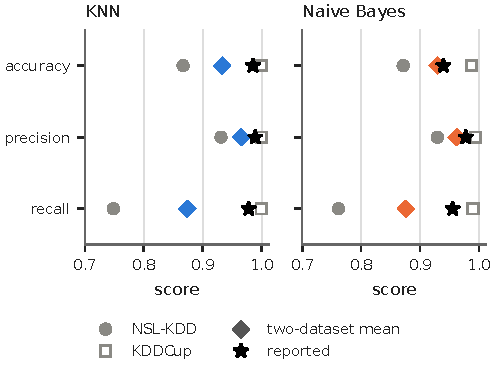
\includegraphics[width=\columnwidth]{figures/fig_paper_comparison.pdf}
  \caption{Accuracy, precision and recall of KNN (left) and Naive Bayes (right) with 8 features on the official NSL-KDD test set, on our KDDCup split, as their mean, and as reported in the reference description. The mean lies below the reported value in every case, and the NSL-KDD result is the lowest of our points.}
  \label{fig:paper_comparison}
\end{figure}

\subsection{Feature selection}\label{sec:feat}
Fig.~\ref{fig:feature_ranking} shows the twelve features with the largest absolute Spearman correlation on each training set. On KDDCup, \texttt{dst\_bytes} ranked \nm{rankCupDstBytes}, \texttt{protocol\_type} ranked \nm{rankCupProtocol}, and \texttt{count} and \texttt{dst\_host\_count} ranked \nm{rankCupCount} and \nm{rankCupDstHostCount}. These are the kinds of features named in the reference description. The KDDCup top eight were \topCup. On NSL-KDD, in contrast, \texttt{dst\_bytes} ranked \nm{rankNslDstBytes} and \texttt{protocol\_type} ranked \nm{rankNslProtocol}, so neither entered the top eight, and \texttt{count} and \texttt{dst\_host\_count} ranked \nm{rankNslCount} and \nm{rankNslDstHostCount}. The NSL-KDD top eight were \topNsl.

\begin{figure*}[t]
  \centering
  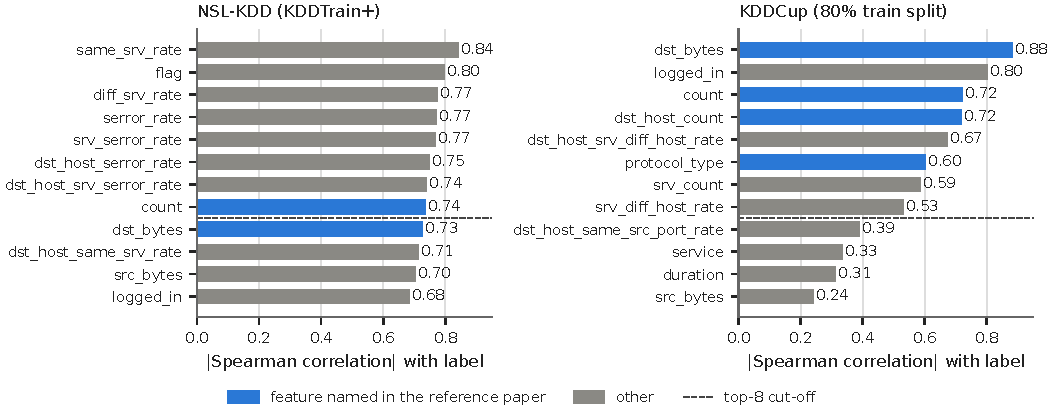
\includegraphics[width=\textwidth]{figures/fig_feature_ranking.pdf}
  \caption{Twelve features with the largest absolute Spearman correlation with the label on the NSL-KDD training set (left) and the KDDCup training split (right). Blue bars mark features named in the reference description, and the dashed line marks the cut-off after the eighth feature. The named features appear above the cut-off on KDDCup but not on NSL-KDD.}
  \label{fig:feature_ranking}
\end{figure*}

\subsection{Performance across setups}
Table~\ref{tab:official} gives the full results on the official split, and Table~\ref{tab:holdout} the accuracy and F1 on the two in-distribution splits. With 8 features on the official split, accuracy ranged from \pc{offAccDtEight} for the decision tree to \pc{offAccNbEight} for NB. With 41 features, KNN, the decision tree and the forests improved, to between \pc{offAccKnnAll} and \pc{offAccDtAll}, whereas NB fell to \pc{offAccNbAll}. The same direction was observed for NB on the holdout split (\pc{nbAccEightHold} to \pc{nbAccAllHold}) and on KDDCup (\pc{nbAccEightCup} to \pc{nbAccAllCup}). All other models reached at least \pc{minAccAllHold} accuracy on the holdout split and \pc{minAccAllCup} on KDDCup with 41 features. On the official split with 41 features, the decision tree (\pc{offAccAllDt}) exceeded the default forest (\pc{offAccAllRf}) and the tuned forest (\pc{offAccAllRft}).
\begin{table*}[t]
\centering
\caption{NSL-KDD official split (train on KDDTrain+, test on KDDTest+), percent. Rec.\ seen and Rec.\ unseen are recall on DoS types present and absent in training.}
\label{tab:official}
\footnotesize
\setlength{\tabcolsep}{2.5pt}
\begin{tabular}{lrrrrrrr}
\toprule
Model & Feat. & Acc. & Prec. & Rec. & F1 & Rec.\ seen & Rec.\ unseen \\
\midrule
KNN & 8 & 86.66 & 93.09 & 74.83 & 82.97 & 87.67 & 31.92 \\
Naive Bayes & 8 & 87.12 & 92.93 & 76.15 & 83.71 & 85.16 & 46.01 \\
Decision Tree & 8 & 84.97 & 92.79 & 70.92 & 80.39 & 86.52 & 18.75 \\
Random Forest & 8 & 85.43 & 92.99 & 71.87 & 81.08 & 87.42 & 19.86 \\
RF (tuned) & 8 & 86.39 & 93.23 & 74.05 & 82.54 & 87.25 & 29.94 \\
\midrule
KNN & 41 & 89.53 & 99.00 & 76.67 & 86.41 & 97.53 & 6.93 \\
Naive Bayes & 41 & 61.78 & 53.95 & 82.06 & 65.10 & 93.36 & 44.26 \\
Decision Tree & 41 & 91.33 & 96.51 & 83.05 & 89.28 & 98.68 & 30.81 \\
Random Forest & 41 & 90.12 & 98.45 & 78.48 & 87.34 & 99.49 & 8.21 \\
RF (tuned) & 41 & 90.59 & 98.93 & 79.20 & 87.97 & 94.83 & 26.97 \\
\bottomrule
\end{tabular}
\end{table*}

\begin{table}[t]
\centering
\caption{Accuracy and F1 (percent) on the two in-distribution 80/20 splits.}
\label{tab:holdout}
\footnotesize
\setlength{\tabcolsep}{2.5pt}
\begin{tabular}{lrrrrr}
\toprule
 & & \multicolumn{2}{c}{NSL-KDD holdout} & \multicolumn{2}{c}{KDDCup} \\
\cmidrule(lr){3-4}\cmidrule(lr){5-6}
Model & Feat. & Acc. & F1 & Acc. & F1 \\
\midrule
KNN & 8 & 97.33 & 96.62 & 99.88 & 99.92 \\
Naive Bayes & 8 & 95.52 & 94.40 & 98.72 & 99.20 \\
Decision Tree & 8 & 97.28 & 96.55 & 99.94 & 99.96 \\
Random Forest & 8 & 97.34 & 96.63 & 99.94 & 99.96 \\
RF (tuned) & 8 & 97.17 & 96.40 & 99.83 & 99.90 \\
SVM & 8 & 97.19 & 96.43 & 99.36 & 99.60 \\
\midrule
KNN & 41 & 99.96 & 99.95 & 99.99 & 100.00 \\
Naive Bayes & 41 & 65.78 & 69.82 & 93.31 & 95.97 \\
Decision Tree & 41 & 99.97 & 99.96 & 99.99 & 99.99 \\
Random Forest & 41 & 99.99 & 99.99 & 100.00 & 100.00 \\
RF (tuned) & 41 & 99.69 & 99.62 & 99.95 & 99.97 \\
SVM & 41 & 99.95 & 99.93 & 99.99 & 99.99 \\
\bottomrule
\end{tabular}
\end{table}


Fig.~\ref{fig:confusion} shows the confusion matrices of KNN and NB with 8 features on the official split and on KDDCup. On the official split, both models produce a substantial number of false negatives, whereas on KDDCup errors are rare for both.

\begin{figure*}[t]
  \centering
  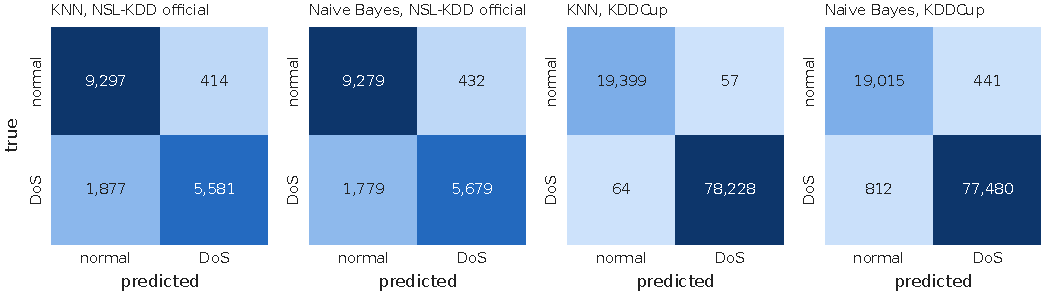
\includegraphics[width=\textwidth]{figures/fig_confusion.pdf}
  \caption{Confusion matrices of KNN and Naive Bayes with 8 features on the official NSL-KDD test set and on the KDDCup split. Cell values are record counts. Missed DoS records dominate the errors on the official split.}
  \label{fig:confusion}
\end{figure*}

\subsection{Unseen attack types}
Fig.~\ref{fig:seen_unseen} compares recall on DoS types seen in training with recall on the unseen types of the official test set. With 8 features, recall on unseen types ranged from \pc{unseenMinEight} to \pc{unseenMaxEight} across the five models, and NB had the highest value. With 41 features the range was \pc{unseenMinAll} to \pc{unseenMaxAll}. For KNN, using all 41 features raised recall on seen types from \pc{seenKnnEight} to \pc{seenKnnAll} but lowered it on unseen types from \pc{unseenKnnEight} to \pc{unseenKnnAll}. The tuned forest reached \pc{unseenRftEight} and \pc{unseenRftAll} with 8 and 41 features, against \pc{unseenRfEight} and \pc{unseenRfAll} for the default forest.

\begin{figure}[t]
  \centering
  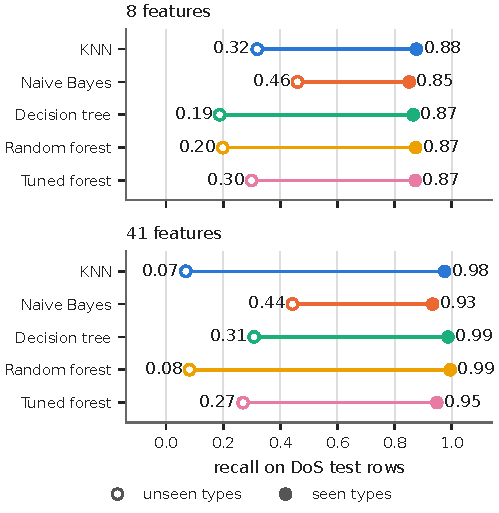
\includegraphics[width=\columnwidth]{figures/fig_seen_unseen.pdf}
  \caption{Recall on unseen (open marker, left end of each segment) and seen (filled marker, right end) DoS types on the official NSL-KDD test set, with 8 features (top) and 41 features (bottom). Every model loses recall on unseen types, and the length of each segment indicates the size of the loss.}
  \label{fig:seen_unseen}
\end{figure}

\subsection{Leave-one-attack-out}
Table~\ref{tab:loao} summarizes the leave-one-attack-out experiment, and Fig.~\ref{fig:loao_heatmap} shows held-out recall for every group. For KNN, the decision tree and the two forests, \nm{loaoUnderHalf} of \nm{loaoN} results had held-out recall below 50\%, whereas recall on seen types was at least \pc{loaoSeenMin} and the false-alarm rate at most \pc{loaoFaMax}. KNN's mean held-out recall was at most \pc{knnLoaoMax} in every setup.
\begin{table*}[t]
\centering
\caption{Leave-one-attack-out, mean over the four held-out groups (percent, one seed). Held-out is recall on the withheld DoS types, Seen is recall on the DoS types kept in training, and FA is the false-alarm rate on normal traffic.}
\label{tab:loao}
\footnotesize
\setlength{\tabcolsep}{2.5pt}
\begin{tabular}{lrrrrrrr}
\toprule
 & & \multicolumn{3}{c}{NSL-KDD} & \multicolumn{3}{c}{KDDCup} \\
\cmidrule(lr){3-5}\cmidrule(lr){6-8}
Model & Feat. & Held-out & Seen & FA & Held-out & Seen & FA \\
\midrule
KNN & 8 & 1.79 & 97.99 & 0.32 & 0.73 & 99.96 & 0.29 \\
Naive Bayes & 8 & 36.46 & 92.44 & 30.87 & 43.84 & 98.80 & 3.50 \\
Decision Tree & 8 & 2.91 & 98.41 & 0.13 & 25.71 & 99.97 & 0.07 \\
Random Forest & 8 & 2.42 & 98.45 & 0.12 & 23.78 & 99.97 & 0.05 \\
RF (tuned) & 8 & 0.47 & 98.23 & 0.21 & 17.69 & 99.74 & 0.05 \\
SVM & 8 & 0.41 & 97.17 & 0.37 & 19.35 & 99.31 & 0.03 \\
\midrule
KNN & 41 & 0.64 & 99.62 & 0.05 & 0.67 & 99.99 & 0.01 \\
Naive Bayes & 41 & 48.67 & 98.68 & 45.61 & 18.58 & 98.86 & 9.86 \\
Decision Tree & 41 & 4.61 & 99.94 & 0.06 & 4.63 & 100.00 & 0.01 \\
Random Forest & 41 & 2.18 & 99.94 & 0.02 & 0.97 & 100.00 & 0.00 \\
RF (tuned) & 41 & 0.93 & 99.80 & 0.22 & 28.84 & 99.33 & 0.04 \\
SVM & 41 & 0.76 & 99.89 & 0.06 & 0.00 & 99.99 & 0.01 \\
\bottomrule
\end{tabular}
\end{table*}


NB showed the highest mean held-out recall, \pc{nbLoaoNslAllRec} on NSL-KDD with 41 features, but with a false-alarm rate of \pc{nbLoaoNslAllFa}; with 8 features the figures were \pc{nbLoaoNslEightRec} and \pc{nbLoaoNslEightFa}. In the extreme case of \texttt{smurf} withheld from NSL-KDD with 8 features, NB flagged \pc{nbSmurfNslRec} of the held-out records and \pc{nbSmurfNslFa} of the normal records. On KDDCup with 8 features, the same group yielded a held-out recall of \pc{nbSmurfCupRec} at a false-alarm rate of \pc{nbSmurfCupFa}. Fig.~\ref{fig:loao_tradeoff} plots held-out recall against false-alarm rate for all results.

\begin{figure*}[t]
  \centering
  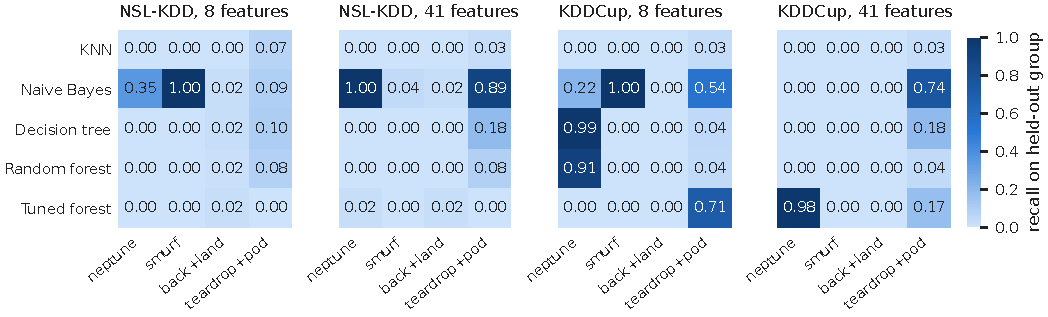
\includegraphics[width=\textwidth]{figures/fig_loao_heatmap.pdf}
  \caption{Held-out recall in the leave-one-attack-out experiment, for each model (rows) and held-out attack group (columns), on NSL-KDD and KDDCup with 8 and 41 features. Recall varies between near zero and near one across groups for the same model.}
  \label{fig:loao_heatmap}
\end{figure*}

\begin{figure}[t]
  \centering
  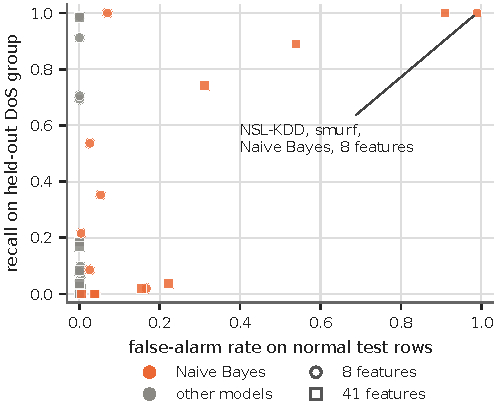
\includegraphics[width=\columnwidth]{figures/fig_loao_tradeoff.pdf}
  \caption{False-alarm rate against held-out recall for all leave-one-attack-out results. Naive Bayes (orange) attains high held-out recall only at the cost of false-alarm rates of up to \pc{nbFaMax}, as at the annotated point, while the other models (gray) cluster at low false-alarm rates and, mostly, at low recall.}
  \label{fig:loao_tradeoff}
\end{figure}

\subsection{Tree models and tuning}\label{sec:tuning}
In leave-one-attack-out evaluation, the advantage of the tuned forest on unseen types did not carry over. Its mean held-out recall exceeded that of the default forest only on KDDCup with 41 features (\pc{loaoCupAllRft} against \pc{loaoCupAllRf}), and was lower on KDDCup with 8 features (\pc{loaoCupEightRft} against \pc{loaoCupEightRf}) and on NSL-KDD (\pc{loaoNslEightRft} against \pc{loaoNslEightRf} at 8 features, \pc{loaoNslAllRft} against \pc{loaoNslAllRf} at 41).

We re-ran the hyperparameter search that produced the tuned settings, using 30 randomized candidates and 3-fold cross-validation, either stratified in the usual way or with each fold withholding one attack group. Fig.~\ref{fig:rf_tuning} shows the outcome over five seeds on the official test set. The best attack-out cross-validated F1 was only \nm{rfTunAoCv}, against \nm{rfTunStdCv} for standard cross-validation. The attack-out configuration reached an unseen-type recall of \nm{rfTunAoU}, against \nm{rfDefAllU} for the default 41-feature forest and \nm{rfTunStdU} for the standard-CV configuration. The attack-out configuration did not exceed the fixed tuned forest on the official test set, whose single-seed unseen-type recall with 41 features was \pc{unseenRftAll}. The search selected settings different from those fixed in the code, which is consistent with a dependence of the forest's random feature choices on column order, itself determined by the correlation ranking.

\begin{figure}[t]
  \centering
  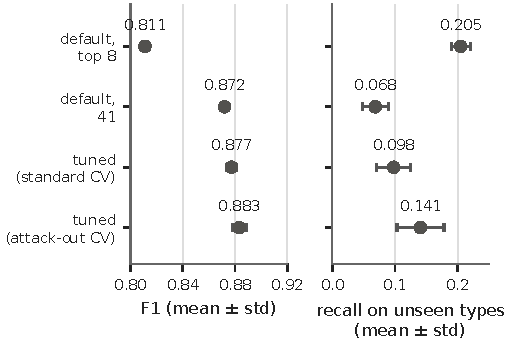
\includegraphics[width=\columnwidth]{figures/fig_rf_tuning.pdf}
  \caption{Mean F1 (left) and mean recall on unseen types (right) with one standard deviation over five seeds, for four random-forest configurations on the official NSL-KDD test set; values are labeled. The attack-out search yields a modest gain in unseen-type recall over the default 41-feature forest.}
  \label{fig:rf_tuning}
\end{figure}

\subsection{Computational cost}
Table~\ref{tab:timing} and Fig.~\ref{fig:timing} report the median training and prediction times. KNN stores the training data, so its training time is small, but its prediction time was \nm{knnPredMin} to \nm{knnPredMax} times that of NB depending on the setup, and \nm{knnPredCupAll} s on KDDCup with 41 features. The median training time of the default forest was \nm{trainRfMin} to \nm{trainRfMax} times that of the decision tree, and for the tuned forest \nm{trainRftMin} to \nm{trainRftMax} times. The decision tree predicted at a speed comparable to NB (ratio \nm{dtPredMin} to \nm{dtPredMax}).
\begin{table*}[t]
\centering
\caption{Median of 5 runs of prediction and training time in seconds, and the ratios of prediction time to Naive Bayes (Pred./NB) and of training time to the Decision Tree (Train/DT). Measured on an 8-core machine under background load.}
\label{tab:timing}
\footnotesize
\setlength{\tabcolsep}{2.5pt}
\begin{tabular}{lrrrrrrrr}
\toprule
 & \multicolumn{4}{c}{NSL-KDD official, 8 features} & \multicolumn{4}{c}{KDDCup, 41 features} \\
\cmidrule(lr){2-5}\cmidrule(lr){6-9}
Model & Pred.\ (s) & Train (s) & Pred./NB & Train/DT & Pred.\ (s) & Train (s) & Pred./NB & Train/DT \\
\midrule
KNN & 0.861 & 0.0193 & 726 & 0.228 & 24.4 & 0.12 & 1{,}771 & 0.185 \\
Naive Bayes & 0.00119 & 0.0138 & 1 & 0.162 & 0.0138 & 0.107 & 1 & 0.166 \\
Decision Tree & 0.00165 & 0.0849 & 1.39 & 1 & 0.00565 & 0.648 & 0.41 & 1 \\
Random Forest & 0.169 & 3.22 & 143 & 37.9 & 0.219 & 11.2 & 15.9 & 17.3 \\
RF (tuned) & 0.206 & 4.18 & 174 & 49.2 & 0.256 & 10.6 & 18.6 & 16.3 \\
\bottomrule
\end{tabular}
\end{table*}


\begin{figure*}[t]
  \centering
  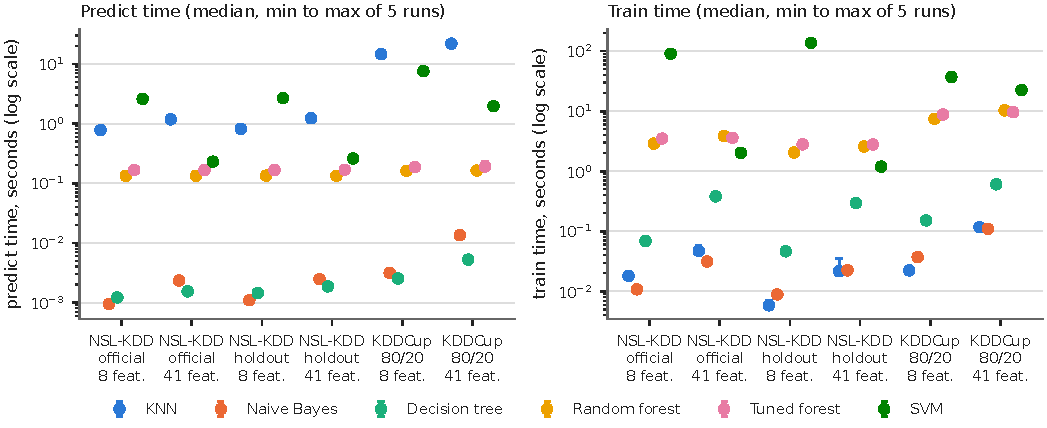
\includegraphics[width=\textwidth]{figures/fig_timing.pdf}
  \caption{Median prediction time (left) and training time (right) in seconds on a logarithmic scale for each model and setup, with minimum--maximum whiskers over five runs. The prediction time of KNN exceeds that of Naive Bayes and the decision tree by orders of magnitude, and the training time of the forests exceeds that of the other models.}
  \label{fig:timing}
\end{figure*}

\section{Discussion}\label{sec:discussion}
\subsection{Research questions}
\emph{RQ1: reproduction.} The reported results were reproduced only in part. On KDDCup the models reached or exceeded the reported metrics, but on the official NSL-KDD test set they fell short, and the two-dataset means were below the reported values for both models (Table~\ref{tab:paper}). The NB discrepancy was small and the KNN discrepancy larger. Because the exact features, $K$ and split of the source study are unknown, the shortfall may reflect differences in protocol rather than a flaw in the original result, and we cannot distinguish these explanations. The Spearman ranking nevertheless recovered the named features on KDDCup, which is consistent with, but does not demonstrate, the use of a similar filter in the source study.

\emph{RQ2: unseen attack types.} Models that achieved near-perfect accuracy on random splits detected few DoS types withheld from training. The pattern appeared on the official split (Fig.~\ref{fig:seen_unseen}) and in the leave-one-attack-out experiment for KNN and the three tree-based models (Table~\ref{tab:loao}). The higher held-out recall of NB was accompanied by high false-alarm rates, so it does not indicate a reliable detector of new attacks. The tuned forest improved unseen-type recall on the official split, but this did not hold in leave-one-attack-out, with one exception. We hypothesize that the unseen types of the official test set resemble some training types more closely than do the groups withheld in our protocol, though we did not test this.

\emph{RQ3: cost.} KNN was the slowest to predict, by a factor of at least \nm{knnPredMin} relative to NB, while the forests were the most expensive to train (Table~\ref{tab:timing}). NB and the decision tree were the cheapest at prediction. Because the measurements were taken under load, ratios are more informative than absolute times.

\subsection{Implications for forensic practice}
An investigator who relies on a classifier validated on a random split may overestimate its ability to flag a new DoS variant. The results suggest reporting recall on attack types withheld from training, jointly with the false-alarm rate, since a high held-out recall can be obtained trivially by flagging most traffic. They also suggest that a lazy learner such as KNN may be impractical for large collections of recorded traffic, given its prediction cost.

\subsection{Comparison with the reference claims}
According to Tundis and Cauteruccio~\cite{tundis2025}, the source study concludes that KNN performs better than NB~\cite{kachavimath2020}. In our two-dataset means the accuracy of KNN was higher than that of NB by less than one percentage point, and on the official NSL-KDD test set NB had the higher accuracy (\pc{nslNbAccuracy} against \pc{nslKnnAccuracy}). The ordering is therefore not robust in our experiments. Matching the reported numbers on KDDCup is comparatively easy, since nearly every model exceeds 99\% on a random split of the 10\% file; agreement on this dataset is thus weak evidence that a method detects attacks in general.

\section{Threats to Validity}\label{sec:threats}
\emph{Internal validity.} The source study was inaccessible, so the exact features, $K$ and split could not be matched; we used $K=5$ and added feature standardization for KNN. No official KDDCup test split exists, so our own 80/20 split replaced it. The leave-one-attack-out experiment used a single seed, so differences of a few points may lie within noise. Timings were measured on a machine under background load. The hyperparameter search is unstable under column order, so the tuned settings are not unique. Categorical features were encoded as alphabetical integers, which imposes an arbitrary order on them and affects their Spearman ranking.

\emph{External validity.} KDDCup'99 and NSL-KDD are old and synthetic, and are criticized in~\cite{tundis2025} as not representing real-world traffic. Only normal and DoS traffic was considered. Our conclusions about unseen attack types may not transfer to current traffic or to other attack families.

\emph{Construct validity.} Held-out recall depends on which groups are withheld; our four groups are a coarse proxy for novel attacks, and they vary widely in difficulty. Reproduction was judged against numbers quoted in a secondary description, and one quoted figure for NB accuracy differs in another source, which we did not verify. Accuracy, precision and recall at a fixed decision threshold do not capture the operating trade-offs that arise in practice.

\section{Conclusion and Future Work}\label{sec:conclusion}
We attempted to reproduce a KNN and NB DoS detector from its secondary description and extended the comparison with tree-based models, a leave-one-attack-out protocol and a timing benchmark. The reported values were approached on KDDCup but not on the official NSL-KDD test set. All models detected few DoS types absent from training, except NB, whose higher recall was accompanied by high false-alarm rates. KNN was the most expensive to apply, and the forests the most expensive to train.

Future work includes adding the planned support vector machine, evaluating across datasets so that training and test data come from different sources, repeating the leave-one-attack-out experiment with multiple seeds, and evaluating on more recent datasets such as UNSW-NB15, which is mentioned in~\cite{tundis2025}.

\bibliographystyle{IEEEtran}
\bibliography{refs}

\end{document}
